% =============================================================
%  Worked example — the 500 kV reference line
%  Carries the representation of Section 3 and the overhead-line
%  parameters of Section 4 through on one line.  All computed values
%  from the two-port evaluation [11]; conductor data [10].
% =============================================================
\subsection{Worked Example: the 500\,kV Reference Line}
\label{sec:reference-line}

Most of the numbers in this report come from one line. It is a 500\,kV,
60\,Hz overhead line of 300\,mi (483\,km) in flat configuration, with three
Bluebird ACSR 2156\,kcmil sub-conductors per phase, 35\,ft phase spacing and
18\,in bundle spacing. The conductor data are the Southwire ACSR
tables~[10] and the resistance is the value at 75\,$^\circ$C.
Table~\ref{tab:ref-line} gives the line and the parameters that follow from
it by~\eqref{eq:ohl-lc}. Section~\ref{sec:natural-power} uses a second
line --- 400\,kV, 50\,Hz, 400\,km --- and says so where it does.

\begin{table}[!ht]
  \centering
  \begin{tabular}{@{}l l r@{}}
    \toprule
    \textbf{Quantity} & & \multicolumn{1}{c}{\textbf{Value}} \\
    \midrule
    $U_n$ & kV & 500 \\
    $f$ & Hz & 60 \\
    $l$ & mi (km) & 300 (483) \\
    Conductor & & $3\times$ Bluebird ACSR \\
    Geometry & ft / in & 35 flat / 18 bundle \\
    \midrule
    $R'$ (75\,$^\circ$C) & m$\Omega$/km & 56.9 \\
    $L'$ & mH/km & 0.891 \\
    $X' = \omega \cdot L'$ & $\Omega$/km & 0.336 \\
    $G'$ & \textmu S/km & 0.05 \\
    $C'$ & nF/km & 12.7 \\
    \bottomrule
  \end{tabular}
  \caption{500\,kV reference line and its per-unit-length parameters}
  \label{tab:ref-line}
\end{table}

At 60\,Hz the susceptance is $\omega \cdot C' = 4.79$\,\textmu S/km, about a
hundred times the conductance, which is the overhead-line case of
Section~\ref{sec:ohl}: the shunt branch is treated as a pure capacitance
throughout.

\subsubsection{Line constants}
\label{sec:ref-constants}

Table~\ref{tab:ref-computed} collects the lumped and distributed constants
of the whole 300\,mi line.

\begin{table}[!ht]
  \centering
  \begin{tabular}{@{}l l r@{}}
    \toprule
    \textbf{Quantity} & & \multicolumn{1}{c}{\textbf{Value}} \\
    \midrule
    $\underline{Z}$ & $\Omega$ & $27.5 + j\,162.2$ \\
    $\underline{Y}$ & mS & $j\,2.31$ \\
    Charging at 1.0\,p.u. & MVAr & 578 \\
    \midrule
    $\alpha$ & Np/km & $1.07 \times 10^{-4}$ \\
    $\beta$ & rad/km & $1.27 \times 10^{-3}$ \\
    $\beta \cdot l$ & $^\circ$ & 35.2 \\
    Wavelength & km & 4936 \\
    $\underline{Z}_w$ & $\Omega$ & $266 - j\,22$ \\
    $P_{nat} = U_n^2 / \mathrm{Re}\left\{\underline{Z}_w\right\}$ & MW & 939 \\
    \bottomrule
  \end{tabular}
  \caption{Computed quantities of the reference line at 300\,mi}
  \label{tab:ref-computed}
\end{table}

\subsubsection{What the lumped approximation costs}
\label{sec:ref-pi-error}

Table~\ref{tab:ref-pi-abs} evaluates all four two-port parameters of this
line at several lengths, once as the nominal $\pi$ of~\eqref{eq:ac-abcd-pi}
and once exactly from~\eqref{eq:ac-abcd-exact}; $\underline{D} =
\underline{A}$ in both. Table~\ref{tab:ref-pi-error} gives the deviations,
and Figure~\ref{fig:ref-model-error}(a) the same comparison continuously
against length~[12].

The four parameters do not degrade together, and the differences matter for
different reasons.

\begin{itemize}
  \setlength{\itemsep}{0.35em}
  \item $\left|\underline{B}\right|$ is the worst and errs high, because the
        nominal $\pi$ keeps the whole series impedance in one branch while
        the real line distributes it among the shunt capacitance. Since
        $P_{max}$ goes inversely with $\left|\underline{B}\right|$, the
        lumped model is \emph{pessimistic} about transfer capability.
  \item $\left|\underline{A}\right|$ and $\left|\underline{C}\right|$ err
        low, and $\left|\underline{A}\right|$ stays within a percent to
        about 350\,mi --- so a model judged on its voltage ratio alone looks
        far better than it is.
  \item $P_{max}$ collects both errors and lands between them: $-7.2$\,\% at
        300\,mi, $-26$\,\% at 600.
\end{itemize}

At 300\,mi the nominal $\pi$ is still usable for voltage work and already
misleading for capability. Beyond about 400\,mi nothing about it is
defensible.

\begin{table}[!ht]
  \centering
  \begin{tabular}{@{}r r r r r r r r@{}}
    \toprule
    \textbf{$l$} & \multicolumn{1}{c}{\textbf{$\beta \cdot l$}}
      & \multicolumn{2}{c}{$\left|\underline{A}\right|$}
      & \multicolumn{2}{c}{$\left|\underline{B}\right|$}
      & \multicolumn{2}{c}{$\left|\underline{C}\right|$} \\
    \cmidrule(lr){3-4}\cmidrule(lr){5-6}\cmidrule(lr){7-8}
    \multicolumn{1}{c}{mi} & \multicolumn{1}{c}{$^\circ$}
      & \multicolumn{1}{c}{$\pi$} & \multicolumn{1}{c}{exact}
      & \multicolumn{1}{c}{$\pi$, $\Omega$} & \multicolumn{1}{c}{exact, $\Omega$}
      & \multicolumn{1}{c}{$\pi$, mS} & \multicolumn{1}{c}{exact, mS} \\
    \midrule
    100 & 11.7 & 0.979 & 0.979 &  54.8 &  54.5 & 0.762 & 0.765 \\
    200 & 23.5 & 0.917 & 0.918 & 109.7 & 106.7 & 1.477 & 1.499 \\
    300 & 35.2 & 0.813 & 0.819 & 164.5 & 154.4 & 2.095 & 2.170 \\
    400 & 46.9 & 0.669 & 0.686 & 219.4 & 195.8 & 2.570 & 2.751 \\
    600 & 70.4 & 0.280 & 0.351 & 329.1 & 252.9 & 2.904 & 3.553 \\
    \bottomrule
  \end{tabular}
  \caption{Two-port parameters of the reference line against length, nominal
           $\pi$ and exact; $\underline{D} = \underline{A}$ throughout~[12]}
  \label{tab:ref-pi-abs}
\end{table}

\begin{table}[!ht]
  \centering
  \begin{tabular}{@{}r r r r r r@{}}
    \toprule
    \textbf{$l$} & \multicolumn{1}{c}{\textbf{$\beta \cdot l$}}
      & \multicolumn{1}{c}{$\left|\underline{A}\right|$}
      & \multicolumn{1}{c}{$\left|\underline{B}\right|$}
      & \multicolumn{1}{c}{$\left|\underline{C}\right|$}
      & \multicolumn{1}{c}{$P_{max}$} \\
    \multicolumn{1}{c}{mi} & \multicolumn{1}{c}{$^\circ$}
      & \multicolumn{1}{c}{\%} & \multicolumn{1}{c}{\%}
      & \multicolumn{1}{c}{\%} & \multicolumn{1}{c}{\%} \\
    \midrule
    100 & 11.7 &  $-0.0$ &  $+0.7$ &  $-0.4$ &  $-0.8$ \\
    200 & 23.5 &  $-0.1$ &  $+2.8$ &  $-1.4$ &  $-3.3$ \\
    300 & 35.2 &  $-0.7$ &  $+6.5$ &  $-3.4$ &  $-7.2$ \\
    400 & 46.9 &  $-2.5$ & $+12.0$ &  $-6.6$ & $-12.4$ \\
    600 & 70.4 & $-20.0$ & $+30.1$ & $-18.2$ & $-25.8$ \\
    \bottomrule
  \end{tabular}
  \caption{Deviation of the nominal $\pi$ from the exact two-port, and the
           resulting error in the maximum transfer at 500\,kV~[12]}
  \label{tab:ref-pi-error}
\end{table}

\begin{figure}[!ht]
  \centering
  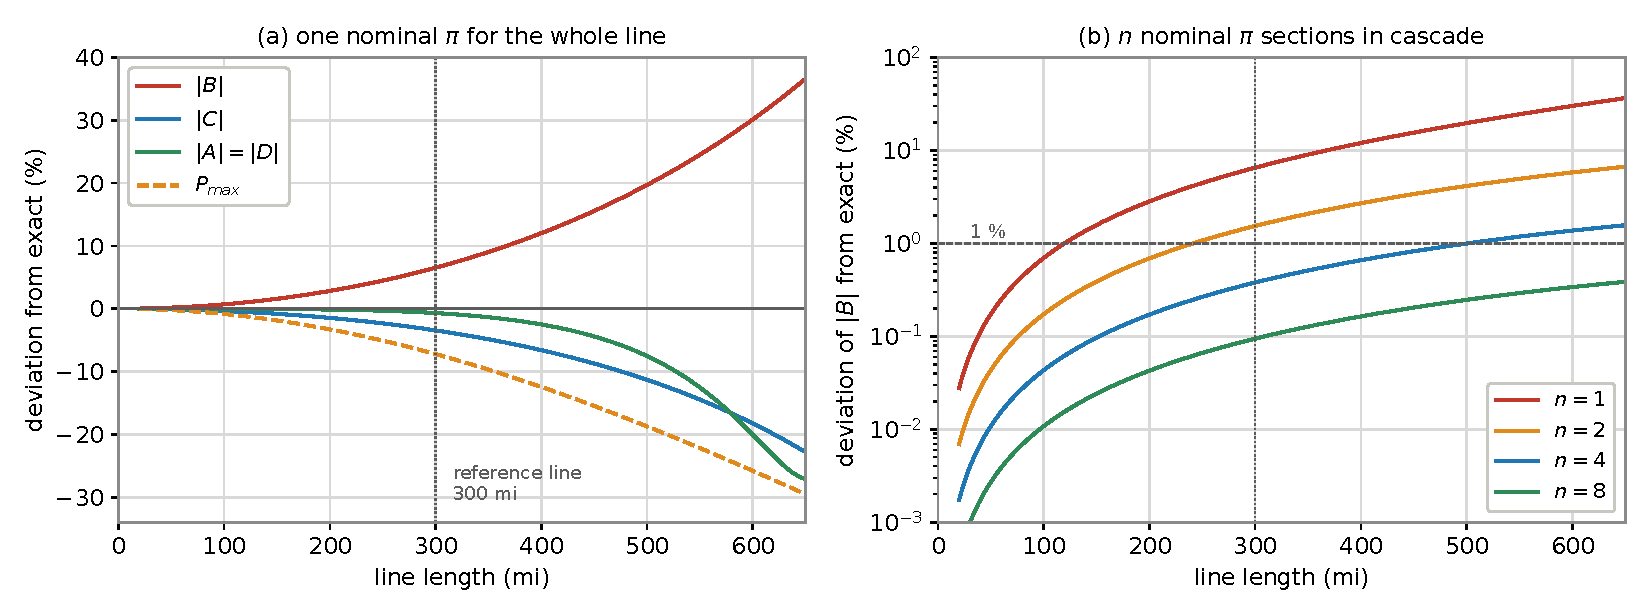
\includegraphics[width=\linewidth]{figures/ac/tp_model_error.pdf}
  \caption{(a) Deviation of the nominal $\pi$ against line length;
           (b) the same deviation of $\left|\underline{B}\right|$ when the
           line is built from $n$ cascaded $\pi$-sections. Both stop short
           of the quarter wavelength, where $\left|\underline{A}\right|$
           passes through zero}
  \label{fig:ref-model-error}
\end{figure}

\FloatBarrier

\subsubsection{Cascading shorter sections}
\label{sec:ref-cascade}

The nominal $\pi$ fails because one lumped section cannot represent a
distribution. The obvious repair is to use more of them: cut the line into
$n$ pieces of length $l/n$, model each as its own nominal $\pi$, and connect
the two-ports in cascade. The chain matrices multiply, so the whole line is
\begin{equation}
  \underline{T} = \left[\underline{T}_{\pi}
    \left(\frac{l}{n}\right)\right]^{n}
  \label{eq:ref-cascade}
\end{equation}
which is one matrix power, not $n$ separate models. Each section is shorter,
so each is a better approximation, and in the limit $n \to \infty$ the
product is the distributed solution of~\eqref{eq:ac-abcd-exact} --- the
cascade is how the exact form is reached from the lumped one.

Table~\ref{tab:ref-cascade} and Figure~\ref{fig:ref-model-error}(b) show the
convergence. The deviation falls with $1/n^2$ once the sections are
electrically short, so each doubling of $n$ buys a factor of four. What
governs the result is the electrical length of a \emph{section}, not of the
line: on this conductor, sections of about 100\,mi hold
$\left|\underline{B}\right|$ inside a percent at any total length, which is
the same 100\,mi that Table~\ref{tab:ref-pi-abs} gives for a whole line.

\begin{table}[!ht]
  \centering
  \begin{tabular}{@{}r l r r r r r@{}}
    \toprule
    \textbf{$n$} & \textbf{section}
      & \multicolumn{5}{c}{deviation of $\left|\underline{B}\right|$, \%} \\
    \cmidrule(lr){3-7}
    & & \multicolumn{1}{c}{100\,mi} & \multicolumn{1}{c}{200\,mi}
      & \multicolumn{1}{c}{300\,mi} & \multicolumn{1}{c}{400\,mi}
      & \multicolumn{1}{c}{600\,mi} \\
    \midrule
     1 & $l$      & $+0.70$ & $+2.83$ & $+6.53$ & $+12.03$ & $+30.13$ \\
     2 & $l/2$    & $+0.17$ & $+0.69$ & $+1.54$ &  $+2.71$ &  $+5.81$ \\
     4 & $l/4$    & $+0.04$ & $+0.17$ & $+0.38$ &  $+0.66$ &  $+1.38$ \\
     8 & $l/8$    & $+0.01$ & $+0.04$ & $+0.09$ &  $+0.16$ &  $+0.34$ \\
    16 & $l/16$   & $+0.00$ & $+0.01$ & $+0.02$ &  $+0.04$ &  $+0.08$ \\
    \bottomrule
  \end{tabular}
  \caption{Nominal $\pi$-sections in cascade: deviation of
           $\left|\underline{B}\right|$ from the exact two-port against the
           number of sections~[12]}
  \label{tab:ref-cascade}
\end{table}

Cascading is not the only repair, and for a plain line it is not the best
one. The equivalent $\pi$ of~\eqref{eq:ac-equivalent-pi} is exact with a
single section, and the correction it applies is not small: on this line at
300\,mi the series branch falls from $27.5 + j\,162.2\,\Omega$ to $24.1 +
j\,152.5\,\Omega$ and the shunt branch rises from 1.156 to 1.193\,mS at each
end, and at 600\,mi from $54.9 + j\,324.4$ to $30.4 + j\,251.0\,\Omega$
against 2.312 to 2.650\,mS. One exact section beats sixteen approximate
ones and costs less to evaluate.

Cascading earns its place where the single equivalent $\pi$ cannot go.

\begin{itemize}
  \setlength{\itemsep}{0.35em}
  \item \textbf{Something is connected part-way along.} A midpoint series
        bank is a two-port cascaded between two half-lines,
        Section~\ref{sec:series-compensation}, and a tapped substation or a
        transposition point divides the line in the same way. The
        equivalent $\pi$ describes a line between its own two ends and
        nothing else.
  \item \textbf{Quantities along the line are wanted.} The voltage profiles
        of Section~\ref{sec:np-profile} are the intermediate port
        quantities of a cascade; a single two-port gives only its terminals.
  \item \textbf{The line is not uniform.} Different conductor, spacing or
        bundle over part of the route gives each part its own matrix, and
        the product handles it with no extra theory. The equivalent $\pi$
        assumes one $\underline{\gamma}$ and one $\underline{Z}_w$ over the
        whole length.
  \item \textbf{A time-domain or frequency-sweep model is wanted.} The
        cascade is a lumped circuit a simulator can integrate directly,
        which is why electromagnetic-transient models still use chained
        sections rather than a closed-form $\cosh$.
\end{itemize}

Where the line is uniform and only its terminals matter, the equivalent
$\pi$ is the right model, and the cascade is a way of understanding where it
comes from. Appendix~\ref{sec:tp-interconnection} sets the cascade beside
the other ways two-ports combine, which are not interchangeable with it.

\subsubsection{The three representations compared}
\label{sec:ref-models}

Table~\ref{tab:ref-models} evaluates the two-port parameters and the crest
of the power-angle curve for the same line under the three representations
of Section~\ref{sec:ac-transmission}. The simplification
of~\eqref{eq:ac-simple} moves the maximum from $81.0^\circ$ to $90^\circ$
and overstates it by 13\,\%; the nominal $\pi$ keeps the angle but
understates the maximum by 7\,\%, because its $\left|\underline{B}\right|$
is too large. At 300\,mi $\left|\underline{A}\right| = 0.82$, so the line is
already far from the single series impedance that~\eqref{eq:ac-simple}
assumes. The numbers follow from the model of
Section~\ref{sec:ac-transmission} implemented in~[11].

\begin{table}[!ht]
  \centering
  \begin{tabular}{@{}l r r r r@{}}
    \toprule
    \textbf{Model} & \multicolumn{1}{c}{\textbf{$\left|A\right|$}}
      & \multicolumn{1}{c}{\textbf{$\vartheta_B$}}
      & \multicolumn{1}{c}{\textbf{$\left|B\right|$}}
      & \multicolumn{1}{c}{\textbf{$P_{max}$}} \\
    & & \multicolumn{1}{c}{$^\circ$} & \multicolumn{1}{c}{$\Omega$}
      & \multicolumn{1}{c}{MW} \\
    \midrule
    Short, lossless & 1.000 & 90.0 & 162.2 & 1541 \\
    Nominal $\pi$   & 0.813 & 80.4 & 164.5 & 1266 \\
    Distributed     & 0.819 & 81.0 & 154.4 & 1364 \\
    \bottomrule
  \end{tabular}
  \caption{Two-port parameters and maximum transfer at 300\,mi, both
           terminals at 1.0\,p.u.}
  \label{tab:ref-models}
\end{table}

\subsubsection{The surrounding system}
\label{sec:ref-scr}

The reactance that appears in~\eqref{eq:ac-simple} is the whole path between
the two internal voltages, not the line:
\begin{equation}
  X_{tot} = X_{th\_s} + X_{tr\_s} + X' + X_{tr\_r} + X_{th\_r},
  \qquad
  X_{th} = \frac{U_n^2}{S_{sc}},
  \qquad
  \mathrm{SCR} = \frac{S_{sc}}{P_n}
  \label{eq:ref-xtot}
\end{equation}
with $X_{th}$ the Thevenin reactance of the system behind a terminal, $X_{tr}$
that of the transformer and $S_{sc}$ the short-circuit level there. Taking the
lossless $P_{max} = U_n^2 / X_{tot}$ with equal systems at both ends and the
transformers neglected, Table~\ref{tab:ref-scr} shows how much of the
capability belongs to the terminals rather than to the line.

\begin{table}[!ht]
  \centering
  \begin{tabular}{@{}l r r r@{}}
    \toprule
    \textbf{SCL, each end} & \multicolumn{1}{c}{\textbf{$X_{th}$}}
      & \multicolumn{1}{c}{\textbf{$X_{tot}$}}
      & \multicolumn{1}{c}{\textbf{$P_{max}$}} \\
    \multicolumn{1}{c}{GVA} & \multicolumn{1}{c}{$\Omega$}
      & \multicolumn{1}{c}{$\Omega$} & \multicolumn{1}{c}{MW} \\
    \midrule
    5      & 50.0 & 253.4 &  986 \\
    10     & 25.0 & 203.4 & 1229 \\
    20     & 12.5 & 178.4 & 1401 \\
    stiff  &  0.0 & 153.4 & 1630 \\
    \bottomrule
  \end{tabular}
  \caption{Effect of the surrounding system on the maximum transfer of the
           300\,mi reference line, $X' = 153.4\,\Omega$, transformers
           neglected}
  \label{tab:ref-scr}
\end{table}

A quarter of the capability of this line into 10\,GVA systems is lost to the
terminals rather than to the line itself, which is why a loadability figure
quoted for a line in isolation is optimistic. The same quantity, normalised
as the short-circuit ratio, is what governs converter performance on a DC
link.

\subsubsection{What this is not}
\label{sec:ref-caveat}

$P_{max}$ is not a transfer capability. It is the crest of the power-angle
curve of an uncompensated line between two stiff systems, reached at an
angle no system is operated at. What the line can actually carry follows
from the thermal rating of the conductors, the permissible voltage drop and
the angular stability margin, and from the contingency case rather than the
intact one. Those limits are the subject of a separate section; the
representation of Section~\ref{sec:ac-transmission} is what they are
evaluated on.

\FloatBarrier
